%% This is file `elsarticle-template-1-num.tex',
%%
%% Copyright 2009 Elsevier Ltd
%%
%% This file is part of the 'Elsarticle Bundle'.
%% ---------------------------------------------
%%
%% It may be distributed under the conditions of the LaTeX Project Public
%% License, either version 1.2 of this license or (at your option) any
%% later version.  The latest version of this license is in
%%    http://www.latex-project.org/lppl.txt
%% and version 1.2 or later is part of all distributions of LaTeX
%% version 1999/12/01 or later.
%%
%% The list of all files belonging to the 'Elsarticle Bundle' is
%% given in the file `manifest.txt'.
%%
%% Template article for Elsevier's document class `elsarticle'
%% with numbered style bibliographic references
%%
%% $Id$
%% $URL: http://lenova.river-valley.com/svn/elsbst/trunk/elsarticle-template-1-num.tex $
%%

%%\documentclass[preprint,12pt]{elsarticle}

%% Use the option review to obtain double line spacing
%% \documentclass[preprint,review,12pt]{elsarticle}

%% Use the options 1p,twocolumn; 3p; 3p,twocolumn; 5p; or 5p,twocolumn
%% for a journal layout:
%%\documentclass[final,1p,times]{elsarticle}
%%\documentclass[final,1p,times,twocolumn]{elsarticle}
%% \documentclass[final,3p,times]{elsarticle}
\documentclass[final,3p,times,twocolumn]{elsarticle}
%% \documentclass[final,5p,times]{elsarticle}
%% \documentclass[final,5p,times,twocolumn]{elsarticle}

%% if you use PostScript figures in your article
%% use the graphics package for simple commands
%% \usepackage{graphics}
%% or use the graphicx package for more complicated commands
\usepackage{graphicx}
%% or use the epsfig package if you prefer to use the old commands
%% \usepackage{epsfig}

%% The amssymb package provides various useful mathematical symbols
\usepackage{amssymb}
%% The amsthm package provides extended theorem environments
%% \usepackage{amsthm}

%% The lineno packages adds line numbers. Start line numbering with
%% \begin{linenumbers}, end it with \end{linenumbers}. Or switch it on
%% for the whole article with \linenumbers after \end{frontmatter}.
%% \usepackage{lineno}

%% natbib.sty is loaded by default. However, natbib options can be
%% provided with \biboptions{...} command. Following options are
%% valid:

%%   round  -  round parentheses are used (default)
%%   square -  square brackets are used   [option]
%%   curly  -  curly braces are used      {option}
%%   angle  -  angle brackets are used    <option>
%%   semicolon  -  multiple citations separated by semi-colon
%%   colon  - same as semicolon, an earlier confusion
%%   comma  -  separated by comma
%%   numbers-  selects numerical citations
%%   super  -  numerical citations as superscripts
%%   sort   -  sorts multiple citations according to order in ref. list
%%   sort&compress   -  like sort, but also compresses numerical citations
%%   compress - compresses without sorting
%%
%% \biboptions{comma,round}

% \biboptions{}


\journal{Nuclear Physics B}

\begin{document}

\begin{frontmatter}

%% Title, authors and addresses

%% use the tnoteref command within \title for footnotes;
%% use the tnotetext command for the associated footnote;
%% use the fnref command within \author or \address for footnotes;
%% use the fntext command for the associated footnote;
%% use the corref command within \author for corresponding author footnotes;
%% use the cortext command for the associated footnote;
%% use the ead command for the email address,
%% and the form \ead[url] for the home page:
%%
%% \title{Title\tnoteref{label1}}
%% \tnotetext[label1]{}
%% \author{Name\corref{cor1}\fnref{label2}}
\author{D. Brandt \fnref{slac}}
\author{R. Agnese \fnref{uof}}
\author{P. Redl \fnref{stanford}}
\author{M. Asai \fnref{slac}}
\author{D. Faiez \fnref{ucb}}
\author{M. Kelsey \fnref{slac}}
\author{E. Bagli \fnref{ferrara}}
\author{A. Anderson \fnref{MIT}}
\author{C. Schlupf \fnref{MIT}}

%% \ead{email address}
%% \ead[url]{home page}
%% \fntext[label2]{}
%% \cortext[cor]{SLAC National Accelerator Laboratory, Menlo Park, CA, USA}
%%\address{Address\corref{cot}}
 \fntext[slac]{SLAC National Accelerator Laboratory, Menlo Park, CA, USA}
 \fntext[uof]{University of Florida, Gainesville, FL, USA}
 \fntext[stanford]{Stanford University, Stanford, CA, USA}
 \fntext[ucb]{University of California Berkeley, Berkeley, CA, USA}
 \fntext[ferrara]{University of Ferrara, Ferrara, Italy} 
 \fntext[MIT]{Massachusetts Institute of Technology, Cambridge, MA, USA}


\title{Semiconductor phonon and charge transport Monte Carlo simulation using Geant4}

%% use optional labels to link authors explicitly to addresses:
%% \author[label1,label2]{<author name>}
%% \address[label1]{<address>}
%% \address[label2]{<address>}

\author{}

\address{}

\begin{abstract}

A phonon and charge transport simulation based on the Geant4 Monte Carlo toolkit is presented. The transport code is capable of propagating acoustic phonons, electrons and holes in cryogenic crystals. Anisotropic phonon propagation, oblique carrier propagation (with or without inter-valley scattering) and phonon emission by accelerated carriers are all taken into account. The simulation successfully reproduces theoretical predictions and experimental observations such as phonon caustics, heat pulse propagation times and mean carrier drift velocities.

Implementation of the transport code using the Geant4 toolkit ensures availability of the transport code to the wider scientific community.

\end{abstract}

\begin{keyword}
%% keywords here, in the form: keyword \sep keyword

%% MSC codes here, in the form: \MSC code \sep code
%% or \MSC[2008] code \sep code (2000 is the default)

\end{keyword}

\end{frontmatter}

%%
%% Start line numbering here if you want
%%
%% \linenumbers


%% The Appendices part is started with the command \appendix;
%% appendix sections are then done as normal sections
%% \appendix

%% \section{}
%% \label{}

\section{Introduction}
\label{sec:Introduction}

We present a Monte Carlo simulation of phonon and charge transport in semiconductor crystals using Geant4. Geant4 is a sophisticated C++ based Monte Carlo simulation toolkit maintained by an international collaboration and freely available under an open source license \cite{Geant-A} \cite{Geant-B}. The toolkit was originally developed in support of High Energy Physics (HEP) experiments and provides functionality for the simulation of the passage of particles through complex geometries and materials. It aims to accurately simulate all matter-particle interactions and has become an important tool both for HEP particle accelerator based experiments building Detector Monte Carlo (DMC) simulations and experiments wishing to estimate backgrounds from environmental or cosmic ray radiation sources \cite{CDMS-D}\cite{Brandt}.

In it's current incarnation, the Geant4 toolkit is entirely focused on free particles and does not take into account crystal physics and conduction/valence band interactions of the low energy charge carriers and phonons relevant to condensed matter physics. This paper documents our effort to build a cohesive Geant4 Condensed Matter Physics Monte Carlo simulation toolkit, G4CMP. The original purpose of this project was to accurately reproduce data from the dark-matter direct detection experiment, Cryogenic Dark Matter Search (CDMS) \cite{CDMS-A}\cite{CDMS-B}\cite{CDMS-C}. The CDMS detectors are cylindrical Ge crystals of approximately size $75$~mm in diameter with a height of $25$~mm \cite{CDMS-E}, cooled to $\sim60$~mK. Dark matter particles may recoil from Ge nuclei via the weak force and thus create phonons and free electron-hole pairs within the crystal \cite{Lindhart}. Electron-hole pairs are drifted to the crystal faces using a small drift field ($\sim$~V/m) where they are collected. Phonons are detected by Transition Edge Sensor (TES) bolometers. We aim to reproduce all of these processes in our Monte-Carlo. 
The phonon and charge transport code described models all physics processes believed to be relevant to phonon and charge collection at cryogenic temperatures. This includes anisotropic phonon transport/phonon focusing, phonon isotope scattering, anharmonic downconversion, oblique carrier propagation (with and without inter-valley scattering) and emission of Luke-Neganov phonons by accelerated carriers. We believe that the resulting G4CMP framework is sufficiently general that it is useful to other experiments employing cryogenic charge or phonon detectors. 

\section{Phonon Transport}
\label{sec:PhononTransport}

Phonon transport was the first component of the G4CMP framework to be developed and early results were presented at LTD-14 \cite{Brandt}. Since the phonon transport code described here is intended for temperatures $T<1$K, scattering off thermally excited background phonons is ignored. Currently, only acoustic phonons are simulated.

\subsection{Anisotropic transport and phonon focusing}
\label{sec:Focusing}

Phonons are quantized vibrations of the crystal lattice. The propagation of phonons is governed by the three-dimensional wave equation \cite{Wolfe}:

\begin{equation}
\label{eq:3DWave}
\rho \omega ^2e_i=C_{ijlm}k_jk_me_l
\end{equation}

where $\rho$ is the crystal mass density, $\omega$ is the phonon frequency, $\vec{e}$ is the polarization vector, $\vec{k}$ is the wave vector and $\vec{C}_{ijml}$ is the elasticity tensor.

For any given wave vector, $\vec{k}$, Eq. \ref{eq:3DWave} has three eigenvalues, $\omega$, and three eigenvectors, $\vec{e}$. These correspond to the three different polarization states \textit{Fast Transverse (FT), Slow Transverse (ST)} and \textit{Longitudinal (L)}. The actual direction and velocity of propagation of phonons is given by the group velocity vector $\vec{v_g} = d\omega/dk$. The group velocity can be calculated by interpreting $\omega$ in Eq. \ref{eq:3DWave} as a function of $\vec{k}$:

\begin{equation}
\label{eq:GroupV}
\vec{v_g}=\frac{d \omega (\vec{k})}{d\vec{k}}=\nabla_k \omega (\vec{k})
\end{equation}

Due to the anisotropy in $C_{ijlm}$, Eq. \ref{eq:GroupV} yields a group velocity $\vec{v_g}$ which is not parallel to the phonon momentum $\hbar\vec{k}$. Instead, phonons are focused onto propagation directions which correspond to the highest density of eigenvectors $\vec{k}$. This focusing gives rise to caustics when observing the energy  distribution resulting from a point-like phonon source isotropic in $\vec{k}$-space. The resulting caustics can be observed using micro-calorimeters \cite{Nothrop}. Figure~\ref{fig:caustics} shows that the caustics simulated by the Geant4 phonon transport code are in good agreement with experimental observations. 

For the purposes of the G4CMP phonon transport code, the wave equation is not solved in real time but rather a look-up table is generated which maps $\vec{k}$ onto $\vec{v_g}$ and bilinear interpolation is used to generate a continuous mapping function. Phonon focusing and methods for solving the three-dimensional wave equations are treated in \cite{Wolfe}. %Wolfe's book \cite{Wolfe}. %For further reading please also consider \ref{fig:caustics}.

\begin{figure}
	\centering
		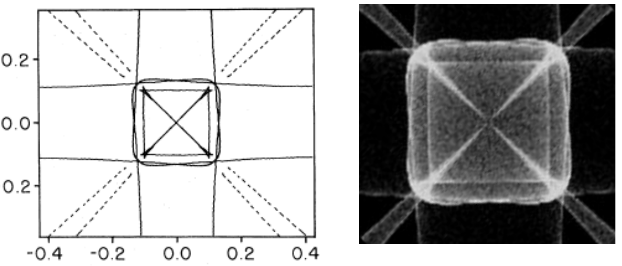
\includegraphics[width=0.5\textwidth]{caustics.png}
	\caption{\textbf{Left:} outline of phonon caustics in Ge as predicted by Nothrop and Wolfe \cite{Nothrop}. \textbf{Right:} Phonon caustics as simulated using the Geant4 phonon transport code. This results is in good agreement with both the theoretical prediction and experimental observations reported by Nothrop and Wolfe \cite{Nothrop} }
	\label{fig:caustics}
\end{figure}

\subsection{Phonon processes}
\label{sec:Processes}

In addition to the phonon equation of motion, which is given by the three dimensional wave equation Eq.~\ref{eq:3DWave}, two processes are relevant to acoustic phonon transport in cryogenic crystals: Isotope scattering and anharmonic down conversion\cite{Tamura1}\cite{Tamura2}\cite{Tamura3}. The scattering and downconversion rates for phonons in the cryogenic crystal are given by \cite{Tamura2}:

\begin{equation}
\label{eq:ScatterRate}
\Gamma_{scatter} = B\nu^4
\end{equation}

\begin{equation}
\label{eq:anhRate}
\Gamma_{anh} = A\nu^5
\end{equation}

where $\Gamma_{scatter}$ is the number of scattering events per unit time, $\Gamma_{anh}$ is the number of anharmonic downconversion events per unit time, $\nu$ is the phonon frequency and $A$, $B$ are constants of proportionality derived from the elasticity tensor. Their value for Ge was discussed in \cite{Brandt} and methods for their derivation can be found in \cite{Tamura1} and \cite{Tamura2}.

The isotope scattering process occurs when a phonon interacts with an isotopic substitution site in the lattice. It is effectively an elastic scattering process during which we assume the phonon momentum vector to be randomized. During this scattering process the phonon polarization state can change freely between the three states $L$, $ST$, $FT$. The branching ratio between the three polarizations is determined by the relative density of allowed states for each polarization.This change between polarization states is often referred to as mode mixing.

The anharmonic down conversion process causes a single energetic phonon to decay into two phonons of reduced energy. This process conserves energy but not momentum, since momentum is exchanged with the crystal lattice. In theory all three polarization states can decay, however, the downconversion rate of $L$-phonons completely dominates the energy evolution of the phonon system, with downconversion events from other polarization states being negligible \cite{Tamura2}.


Eqs. \ref{eq:ScatterRate} and \ref{eq:anhRate} show that both process rates strongly depend on phonon energy $\hbar \nu$. High energy phonons ($\nu$ of order THz) start out in a diffusive regime with high isotope scattering and downconversion rates and mean free paths of order microns. Once a few downconversion events have occurred, phonon mean free paths increase to be of order the size of a typical CDMS detector ($\sim0.1$~m). This transition from a diffuse to a ballistic transport mode is commonly referred to as ``quasi-diffuse'' and controls the time evolution of phonon heat pulses. Simulation of heat pulses using our Geant4 transport code was described in \cite{Brandt} and shows good agreement with experiment. Anharmonic downconversion and isotope scattering are well understood and are discussed in great detail in the literature \cite{Tamura1}\cite{Tamura2}\cite{Wolfe}\cite{Tamura3}.




\section{Charge Transport}
\label{sec:ChargeTransport}

At present, the charge transport component of the G4CMP framework only includes
transport in germanium. For charge carrier transport in germanium, there are
two processes to consider: acceleration by an applied electromagnetic field,
and emission of Neganov-Luke phonons.

When an incoming particle scatters in the germanium crystal, electron-hole
pairs are produced. In the example of the CDMS dark matter detectors, the
charge carriers are drifted by an external electric field to the surfaces of
the detector. 

\subsection{Neganov-Luke Phonons}
As the charge carriers are accelerated through the crystal, they emit phonons
in a process that is analogous to Cerenkov radiation.
\subsubsection{Holes}
Charge carrier-hole scattering is an elastic process, conserving energy and
momentum.

\begin{figure}[htpb]
    \centering
%    \includegraphics[width=.5\textwidth]{scatter}
    \caption{A charge carrier has initial wavevector $\vec{k}$ and emits a
    Neganov-Luke phonon with wavevector $\vec{q}$ \cite{Leman}}.
    \label{fig:scatter}
\end{figure}

From conservation of energy and momentum, $k'^2 = k^2 + q^2 - 2kq\cos{\theta}$
and $q = 2(k\cos{\theta} - k_L$, with $k_L$ defined as $k_L = mv_L/\hbar$,
where $v_L$ is the longitudinal phonon phase speed. Solving for $\phi$,
\begin{equation}
    \cos{\phi} = \frac{k^2 - 2k_s(k\cos{\theta} - k_s) - 2(k\cos{\theta} -
k_s)^2}{k\sqrt{k^2 - 4k_s(k\cos{\theta} - k_s})}
    \label{eq:scatterangle}
\end{equation}
Where $k_L = mv_L/\hbar$. Using Fermi's Golden Rule, we can determine a
scattering rate \cite{Leman},
\begin{equation}
    1/\tau = \frac{v_Lk}{3l_0k_L}\left(1-\frac{k_L}{k}\right)^3
    \label{eq:rate}
\end{equation}
With an angular distribution of,
\begin{equation}
    P(k,\theta) d\theta =
    \frac{v_L}{l_0}\left(\frac{k}{k_L}\right)^2\left(\cos{\theta}-\frac{k_L}{k}\right)^2\sin{\theta}d\theta
    \label{eq:ang-dist}
\end{equation}
Where $0\le\theta\le\arccos{k_L/k}<\pi/2$ and $l_0$ is a characteristic
scattering length defined as $l_0 = \frac{\pi\hbar^4\rho}{2m^3C^2}$ with C
being the deformation potential constant for Ge \cite{Leman}.

\subsubsection{Electrons}
The effective mass of the hole in germanium is a scalar, so its
propagation is simple. The electron, however, has a tensor effective mass.
\begin{figure}[htpb]
    \centering
 %   \includegraphics[width=.5\textwidth]{gebands}
    \caption{Conduction and valence bands in Ge. At present, the G4CMP
    framework only simulates electrons propagating through the L conduction
band. At sufficiently low temperature and applied field, this should match
reality well \cite{Leman}.}
    \label{fig:gebands}
\end{figure}

For a coordinate system with one axis aligned with the principle axis of the
conduction valley, the electron's equation of motion is,
\begin{equation}
    \frac{eE_i}{m_i} = \frac{dv_i}{dt}
    \label{el_eq_mtn}
\end{equation}

However, to simplify the electron propagation, we transform to a coordinate
system in which the constant energy surfaces are spherical. In that space,
$v_i^* = v_i/\sqrt{m_c/m_i}$, where $m_c$ is given by $3/m_c = 1/m_\parallel +
2/m_\perp$. And so,

\begin{equation}
    \frac{eE^*_i}{m_c} = \frac{dv_i^*}{dt}
    \label{el_eq_mtn1}
\end{equation}

Once the coordinate system is rotated into the conduction valley frame, a
Herring-Vogt transformation is then applied,
\begin{equation}
    T_{HV} = \left( \begin{array}{ccc}
                    \sqrt{\frac{m_c}{m_{\parallel}}} & 0 & 0 \\
                    0 & \sqrt{\frac{m_c}{m_{\perp}}} & 0 \\
                    0 & 0 & \sqrt{\frac{m_c}{m_{\perp}}}\end{array}\right)
    \label{HV}
\end{equation}

From this space, the same recipe that applied to holes for propagation and
Neganov-Luke phonon emission can be followed for electrons. One potential issue
is the back-transform into real space. Because the HV matrix is not unitary, it
wont conserve energy. To mitigate the issue, the phonon's momentum magnitude is
kept from the HV space and the back-transform is only used to determine the
angular distribution \cite{Leman}.





\subsection{Inter Valley Scattering}
\label{sec:InterValley}


\begin{figure}
	\centering
		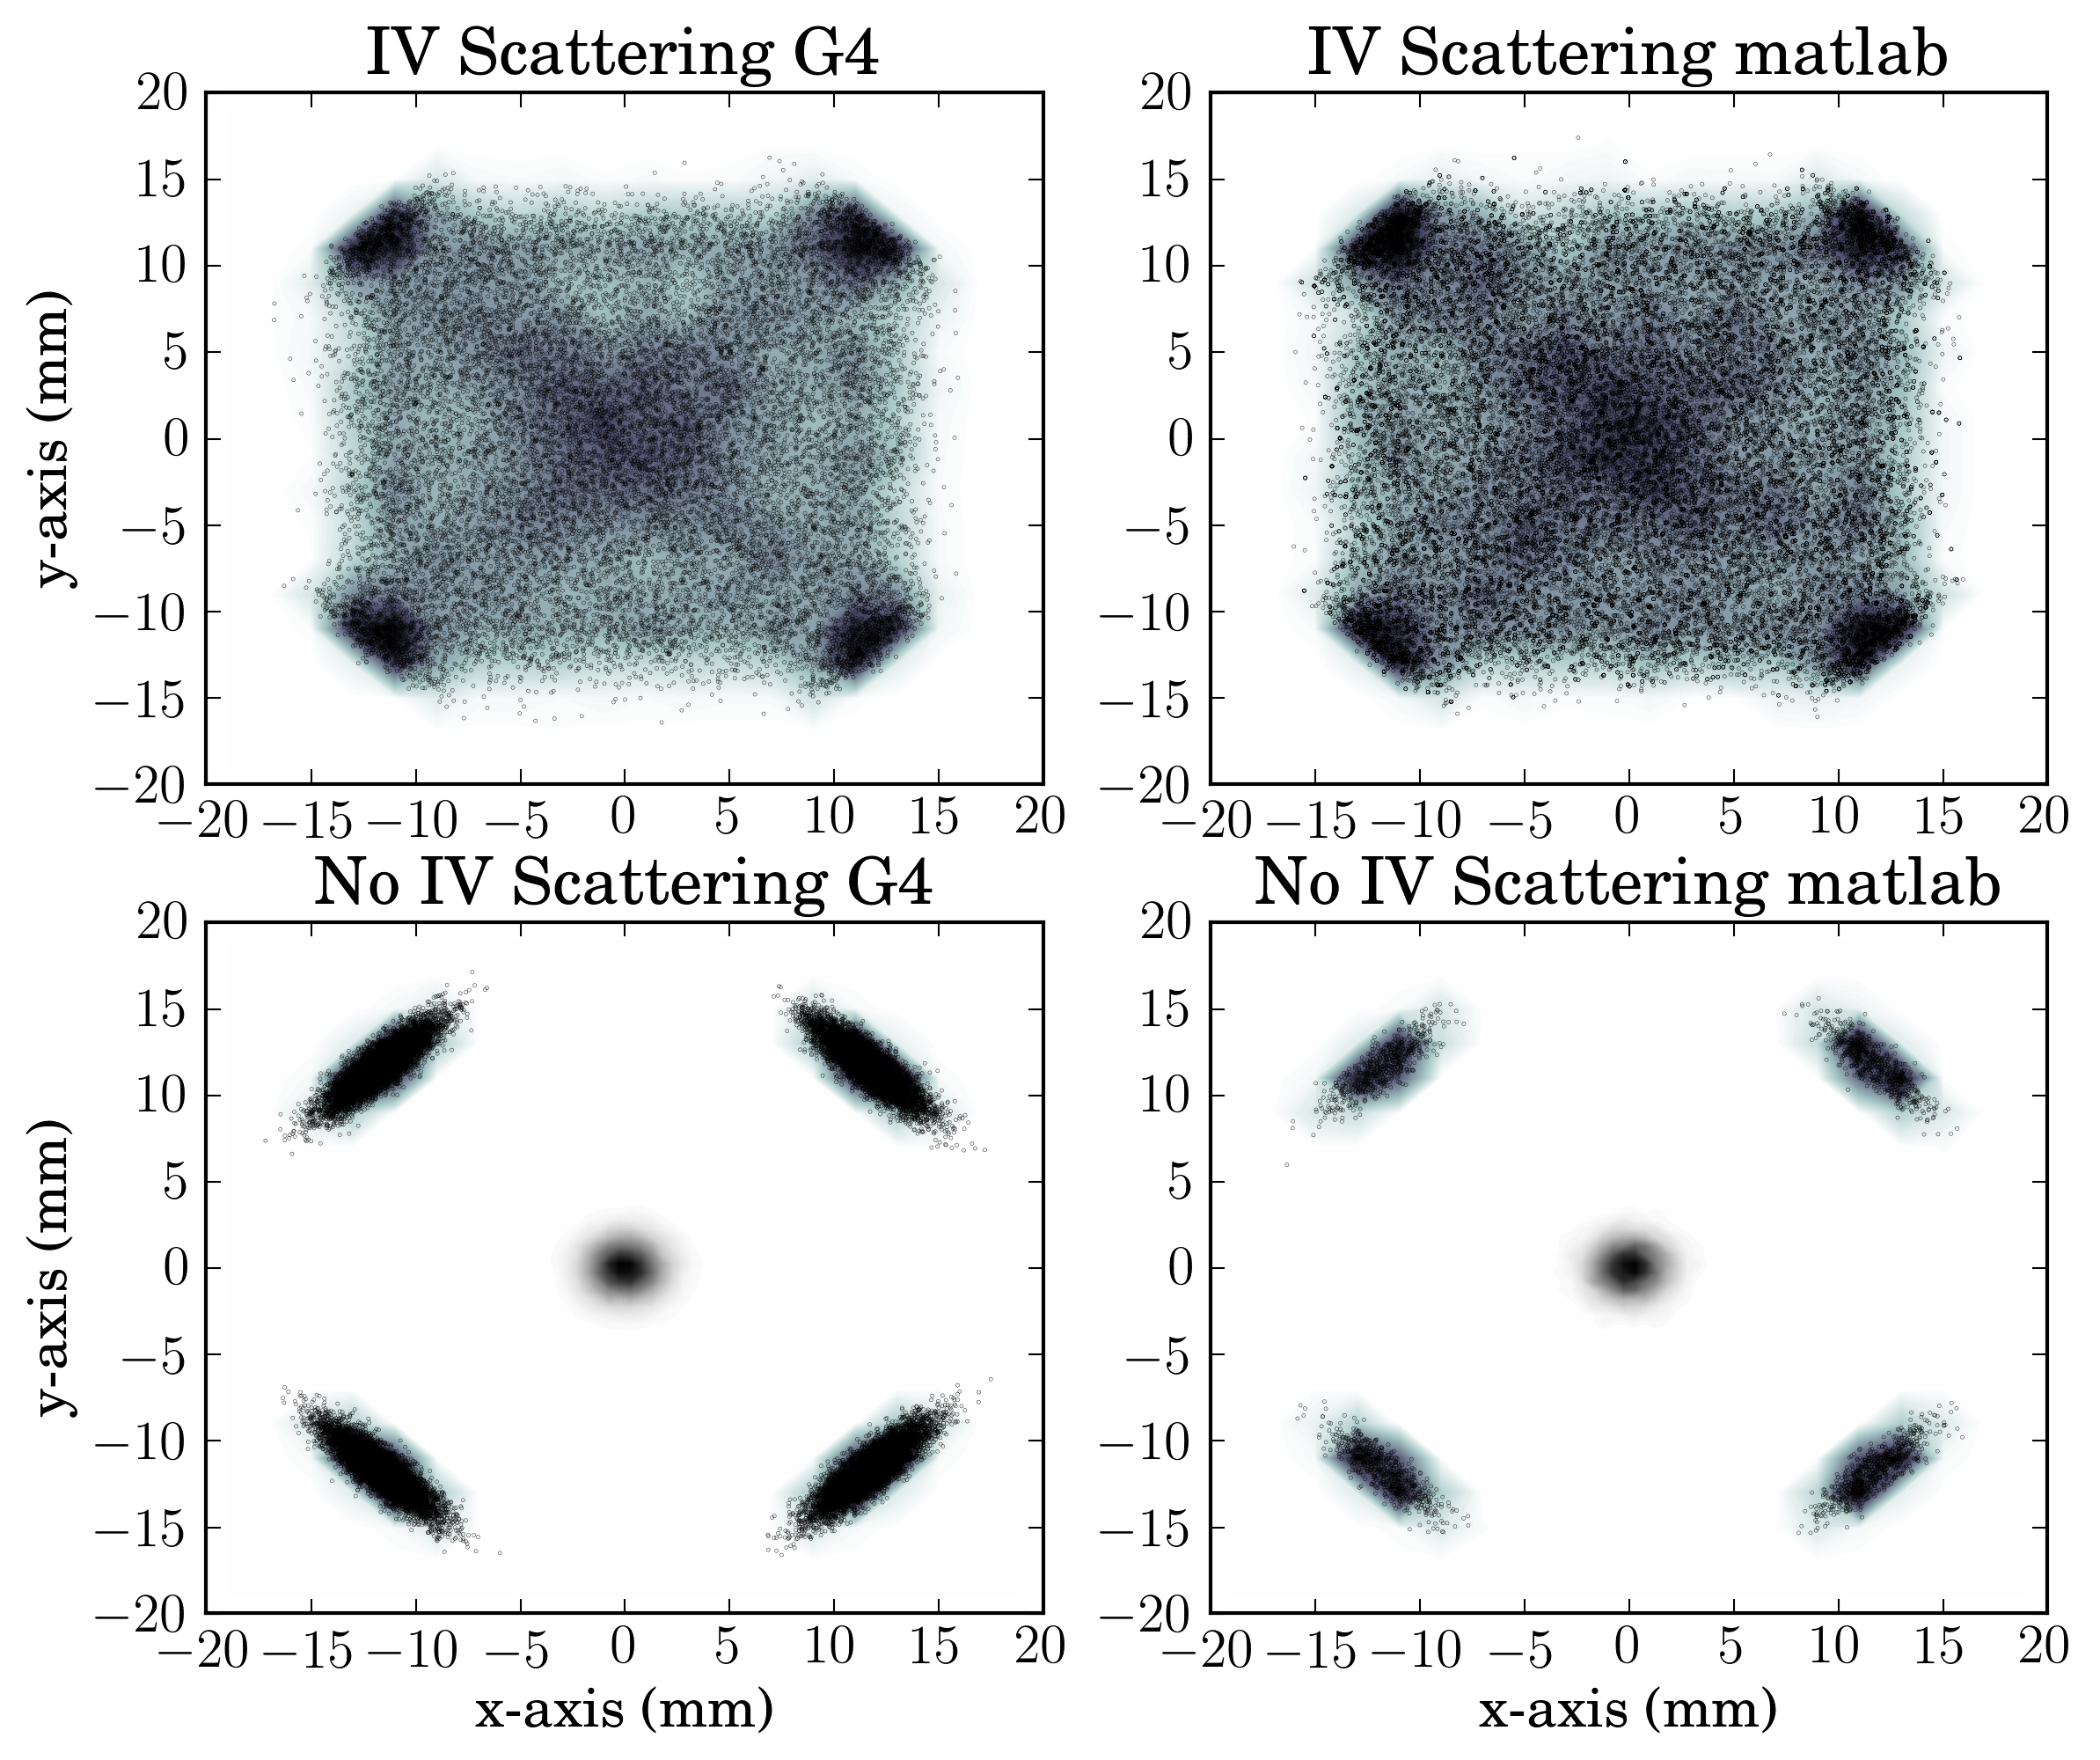
\includegraphics[width=1.0\textwidth]{intervalley.png}
	\caption{\textbf{Left:} Geant4 simulations \textbf{Right:} legacy MATLAB simulations. \textbf{Top Row:} Simulations with inter-valley scattering turned on, \textbf{Bottom Row:} Simulations with inter-valley scattering turned off, including hole transport through the crystal.}
	\label{fig:intervalley}
\end{figure}

Electron propagation as discussed in the previous section, has one particularly interesting feature that electrons propagate through the crystal in one of four distinct valleys \cite{Cabrera,Leman}. Electrons are not bound to those valleys permanently, however, and can scatter between valleys. This process is known as inter-valley scattering and occurs in one of two ways: 1. an electron scatters of the lattice or 2. of an impurity in the crystal structure \cite{iv}. The rate for both processes is dependent on the electric field strength with lattice scattering being the dominant factor in larger fields ($\gtrsim$5~V/m), while impurity scattering dominates in lower fields ($\sim$1~V/m). The EDELWEISS \cite{edelweiss} collaboration determined the scattering rates as a function of the electric field for typical Ge crystals \cite{iv}. We use the results obtained in these studies to set the inter-valley scattering amplitude in the Geant4 framework and compare it to previous implementations of the charge transport code \cite{Cabrera,Leman}. The result of electrons and holes propagating through 2.54~cm of Ge in an 0.5~V/m electric field is shown in Figure~\ref{fig:intervalley}. The top two panels show the result with inter-valley scattering turned on while the bottom two panels show the result for inter-valley scattering turned off. The panels on the right show the results for the legacy simulation \cite{Cabrera,Leman} with somewhat less statistics than the Geant4 simulations. The bottom two panels also show the hole transport through the crystal with the result being the gray contour in the center. 


\section{Conclusion}
\label{sec:Conclusion}

%\begin{itemize}
%  \item presented Monte Carlo transport code capable of propagating e-/h+/ph
%  \item good agreement with experiment
%  \item easily adaptable for other crystals
%  \item implemented in Geant4, so available freely
%\end{itemize}
 
 
We presented Monte Carlo transport code capable of propagating phonons on a cryogenic crystal lattice (Section \ref{sec:PhononTransport}) as well as drifting electron/hole pairs, taking into account conduction band anisotropy (Section \ref{sec:ChargeTransport}). The results produced by the transport code are in good agreement with experiment, reproducing phonon caustics and carrier drift velocity with acceptable accuracy. It was shown that this code reproduces heat pulse propagation and dispersion in cryogenic Ge crystals with acceptable accuracy in \cite{Brandt}. The entire transport code is written in Geant4 and is easily adaptable for crystals other than Ge provided that the Voigt-contracted elasticity tensor and effective carrier masses are known. The Geant4 framework makes it possible to enhance and extend the code presented here. The phonon transport code is already freely available as part of the examples provided with  Geant4 v9.6p02, and newer. 
We hope that the work presented here will establish Geant4 as a tool in condensed matter physics and cryogenic calorimeter design as well as motivating others to add to the G4CMP framework.


%% References
%%
%% Following citation commands can be used in the body text:
%% Usage of \cite is as follows:
%%   \cite{key}          ==>>  [#]
%%   \cite[chap. 2]{key} ==>>  [#, chap. 2]
%%   \citet{key}         ==>>  Author [#]

%% References with bibTeX database:

%\bibliographystyle{model1-num-names}
%\bibliographystyle{phjcp}
\begin{thebibliography}{99}

\bibitem{Geant-A}
J. Allison et al., {\it IEEE Transactions on Nuclear Science} \textbf{53}, 270 - 278, (2006).

\bibitem{Geant-B}
S. Agostinelli et al., {\it Nuclear Instruments and Methods A} \textbf{506}, 250 - 303, (2003).

\bibitem{CDMS-D}
D.S. Akerib et al., {\it Phys. Rev. D} \textbf{72},(2005).

\bibitem{Brandt}
D. Brandt et al., {\it Journal of Low Temperature Physics} \textbf{167}, 485 - 490, (2011).

\bibitem{Lindhart}
Smith, P.F. and Lewin, J.D., {\it Phys.Rept.} \textbf{187}, 203, (1990).

%\bibitem{Enss}
%C. Enss, {\it Cryogenic Particle Detection },Springer Verlag, Germany (2005)

\bibitem{CDMS-A}
Z. Ahmed et al., {\it Science} \textbf{327}, 1619, (2010).

\bibitem{CDMS-B}
Z. Ahmed et al., {\it Phys. Rev. D} \textbf{84}, 011102, (2011).

\bibitem{CDMS-C}
C. Collaboration et al., {\it arxiv astro-ph.CO} \textbf{1304.4279},(2013)

\bibitem{CDMS-E}
R. Agnese et al., {\it arxiv astro-ph} \textbf{1305.2405},(2013)

%\bibitem{Sanglard}
%V. Sanglard et al., {\it Phys. Rev. D.} \textbf{71}, 122002, (2005).

%\bibitem{Lang} %CRESST
%Rafael F. Lang and Wolfgang Seidel, {\it N. J. Phys} \textbf{11}, 105017, (2009).

%\bibitem{Arnaboldi}%CUORE
%C. Arnaboldi et al., {\it NIM A} \textbf{3}, 775, (2004).


\bibitem{Brink}
P. Brink et al., {\it NIM A} \textbf{2}, 414, (2006)

%\bibitem{Hurley}
%D.C. Hurley and J.P. Wolfe, {\it Phys. Rev. B} \textbf{32}, 2568, (1985)

\bibitem{Nothrop}
G.A. Nothrop and J.P. Wolfe, {\it Phys. Rev. Lett.} \textbf{19}, 1424, (1979)

\bibitem{Tamura1}
S. Tamura, {\it J. Lo. T. Phys.} \textbf{93}, 433, (1993)

\bibitem{Tamura2}
S. Tamura, {\it Phys. Rev. B.} \textbf{48}, 13502, (1993)

\bibitem{Wolfe}
J.P. Wolfe, {\it Imaging Phonons, Chapter 2},42, Cambridge University Press, United Kingdom (1998) 

\bibitem{Tamura3}
S. Tamura,{\it Phys. Rev. B.} \textbf{31}, (1985)

\bibitem{Leman}
S. W. Leman, {\it Rev. Sci. Instrum.} \textbf{83}, 091101, (2012).

\bibitem{Cabrera}
Cabrera, B. et al. , {\it arXiv},  Oblique propagation of electrons in crystals of germanium and silicon at sub-Kelvin temperature in low electric fields

\bibitem{iv}
Broniatowski, A., {\it Journal of Low Temperature Physics}, \textbf{167}, (2012)

\bibitem{edelweiss}
Juillard, A., {\it Journal of Low Temperature Physics}, \textbf{151}, (2008) 
%\bibitem{McCarthy}
%K.A. McCarthy et al., {\it These procedings},(2011)

%\bibitem{Anderson}
%A. Anderson et al., {\it These procedings},(2011)


\end{thebibliography}

%% Authors are advised to submit their bibtex database files. They are
%% requested to list a bibtex style file in the manuscript if they do
%% not want to use model1-num-names.bst.

%% References without bibTeX database:

% \begin{thebibliography}{00}

%% \bibitem must have the following form:
%%   \bibitem{key}...
%%

% \bibitem{}

% \end{thebibliography}


\end{document}

%%
%% End of file `elsarticle-template-1-num.tex'.
